\chapter{SysML and SCADE}
\label{sec:sysML-Scade}

\section{Description of the approach}

Diagram \ref{fig:SysML_SCADE_Toolchain} illustrates the most important components and operational relationships of a system and software modeling toolchain based on SysML, Papyrus, SCADE and Eclipse. 
All components and links shown with solid lines are available, while the dashed ones are intended to be implemented within the openETCS project. 


\begin{figure}[htbp]
	\centering
		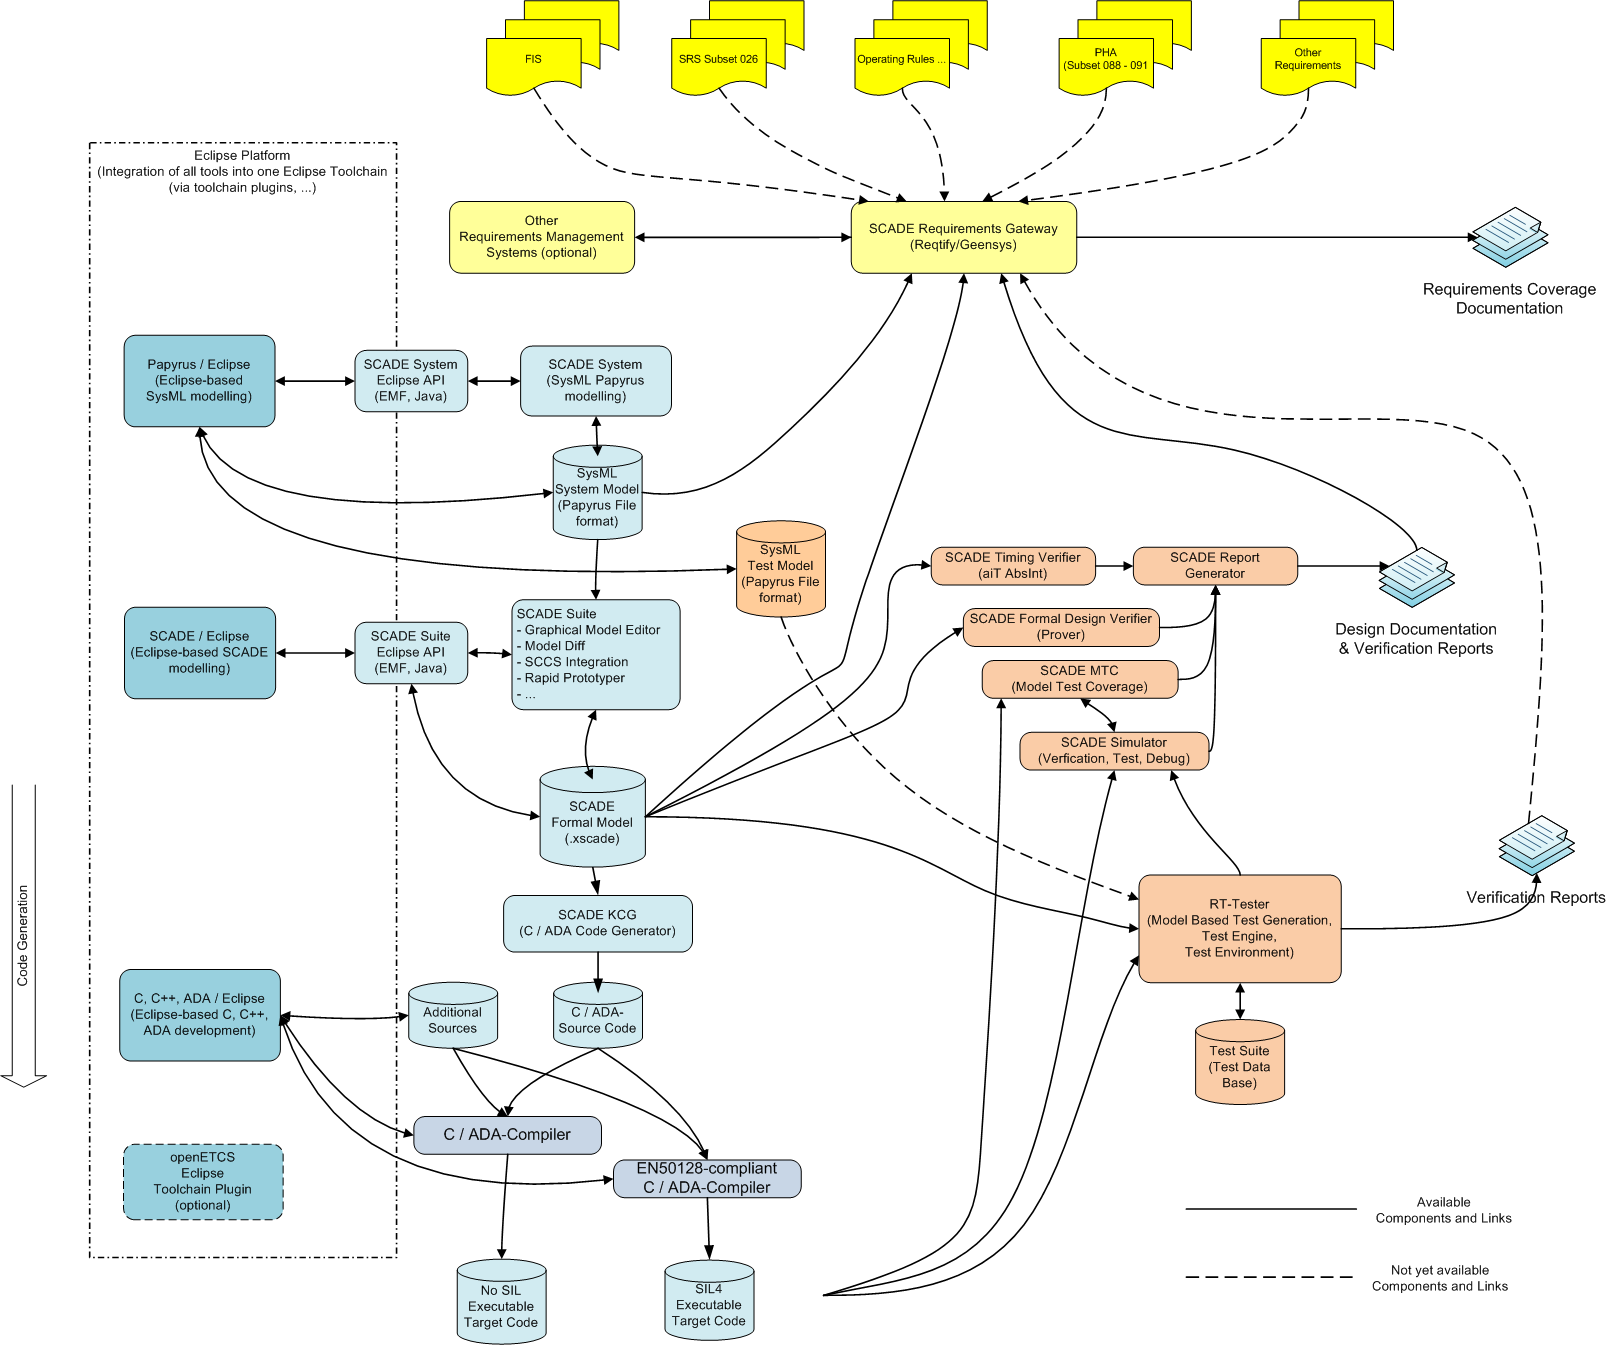
\includegraphics[width=1.10\textwidth]{images/SysML_SCADE_Toolchain.png}
	\caption{SysML SCADE Toolchain}
	\label{fig:SysML_SCADE_Toolchain}
\end{figure}


The diagram colors are chosen related to the colors in figure \ref{fig:main_process}: 

\begin{itemize}
	\item Requirements and requirements management components in yellow
	\item "Blue" openETCS design process ( see figure \ref{fig:main_process}) elements in light and dark blue
	\item Eclipse is painted dark blue
	\item Verification elements in red
\end{itemize}

Within the following paragraphs and subsections a short description of this approach will be given by walking through the tool chain and the design process. 

\subsection{Requirements management}
\label{sec:RequirementsManagement}

The SCADE Requirements Management Gateway is based on Reqtify from Geensoft / Dassault Systems and serves to collect and link all requirements from the openETCS input documents and related objects as design and verification documents, model and source code artifacts, test cases, test protocols etc. It supports impact analyses and generates requirements traceability and requirements coverage reports. 
If needed for the openETCS process, it can be complemented with other requirement management systems and already comes with interfaces to these. Because ProR bases upon the ReqIF file format, and one working principle of Reqtify is to access any type of requirement files via configurable import/export filters, an intergration with ProR is achieveable with little effort. 


\subsection{Semi-formal System and Subsystem Modeling with SCADE System / Papyrus}
\label{sec:SemiformalModelling}

SCADE System is an integration of Papyrus into the SCADE IDE intended for SysML system modeling. It allows to modelize the interactions and hierarchical dependencies between the various parts of a complex system through design elements representing functions, data and interfaces. 
 
The idea is to model system structures, data types / data dictionaries, inputs, outputs, interfaces and relationships between blocks with SysML and transfer it to native SCADE for behavioral modeling automatically. Since Papyrus and SCADE System are using the same file formats, there is no prevention of using all SysML capabilities that Papyrus supports, but in this case without automatic transfer to native SCADE. 

SCADE System supports SysML Block Definition Diagrams (BDD) and	Internal Block Diagrams (IBD).

More details about the relationship between Papyrus and SCADE System: 

\begin{enumerate}
	\item SCADE System 2.x incorporates Papyrus 0.9, but SCADE System is more than Papyrus, as outlined in the following list. SCADE System 3.x (Mar 2014) will be based on Papyrus 0.10.
	
	\item SCADE System enhances Papyrus with functionalities on top: 
	
	\begin{itemize}
		\item Report Generator: Generation of design documents out of the SysML model
		\item Model Check: user expandable checker on SysML models (OCL rule checking, …)
		\item Model Diff: Semantic comparison of models
		\item Interface to requirements management (Reqtify)
		\item Synchronization with SCADE Suite: Mainly blocks and functions with their structure, interfaces, flowports and data types can be transferred to SCADE Suite.   
	\end{itemize}
	
	\item The idea of SCADE System is to ease the work for system and software architects.  SCADE Systems users don’t need so deep knowledge and experience of UML, SysML and …profiles as native Papyrus requires, so that architects or rail engineers, that are not UML experts, are able to work with. Therefore, SCADE System tailors Papyrus in several aspects:
	
	\begin{itemize}
		\item Cleaned up views and user interface and less chances of doing things wrong compared with native Papyrus.
		\item Support for designing blocks (BDD, IBD), relationships and data flows/interfaces between them (as Papyrus).
		\item Support for data types, data dictionaries (as Papyrus).
		\item Allocation of functions (as Papyrus).
	\end{itemize}
	
	\item Actually, SCADE System does not support behavior modeling, but has it on the road map for the next year.
	\item SCADE System uses the same file formats as Papyrus, so that SCADE System and Papyrus files are exchangeable in both directions. SCADE System simply hides SysML artifacts it does not support. This gives the opportunity for:
	
	\begin{itemize}
		\item Using SCADE System for non-UML/SysML experts (architects and rail engineers)
		\item Using Papyrus for UML/SysML experts software experts
	\end{itemize}
	
	\item For integration with Eclipse, SCADE System (as well as SCADE Suite) comes with an Eclipse EMF API including the enhancements on top of Papyrus
\end{enumerate}

With the exception of the synchronization with SCADE Suite, the mentioned easements and enhancements may also be achievable with Papyrus by tailoring and added functionality.
For openETCS, behavioral modeling seems to be necessary for a rather complete model on SysML level. 
Therefore, SCADE System, because ready to use right now, could be chosen for architectural modeling and SSRS matters at the beginning and then continued with Papyrus, when a tailored Papyrus variant becomes available.  

\subsection{Formal Modeling with SCADE Suite}
\label{sec:FormalModellingwithSCADESuite}

SCADE Suite integrates all modeling, verification and supporting SCADE tools under the roof of the SCADE IDE. The components relevant for descending part of the development "`V"' process are

\begin{itemize}
	\item SCADE Suite Editor (Graphical and textual modeling)
	\item SCADE Requirements Gateway Integration (Linking of model artifacts with requirements)
	\item SCADE Model Check (model syntax check)
	\item SCADE Model Diff (model comparison)
	\item SCADE Simulator (graphical debugging, simulation and testing) 
	\item SCADE Rapid Prototyper (quick control and display elements for rapid prototyping, optional)
	\item SCADE Code Generator KCG (C / ADA code generation)
	\item SCADE Reporter ( (Design) report generator)
\end{itemize}

The most important tools for modeling are editor and code generator. The others mentioned are mainly verification tools, but very useful and practically indispensable for agile development.

At least, to cover all elements of the "blue" design process in figure \ref{fig:main_process} a C / C++ / ADA compiler is required. 
For building not safety-relevant executables any C-Compiler (gnu c, ...) is suitable, for safety relevant executables the compiler must be compliant with EN50128.   

\subsection{Model Verification}
\label{sec:SysML_SCADE_ModelVerification}

The verification of openETCS SCADE models can be performed with the "`red"' components shown in diagram \ref{fig:SysML_SCADE_Toolchain}. Most of them are part of SCADE System or SCADE Suite:

\begin{itemize}
	\item SCADE Simulator: The SCADE Simulator should be used in an agile iterative development process for a steady accompanying verification of the modeling work. Simulator test scripts allow executing verification suites for the models automatically. Via its automation and co-simulation interface it is able to be integrated in the openETCS tool chain. 
	\item  SCADE Model Test Coverage MTC: The MTC serves to determine structural model test coverage while executing test scenarios. Instead of measuring code coverage on the generated code, it works on the model structure directly. The MTC tool is automatable. 
	\item SCADE Design Verifier: The verifier performs formal proving and bases upon a model checker from from Prover Technology AB.  
	\item SCADE Timing Verifier: Execution timing verification based on aiT from AbsInt.
	\item SCADE Report Generator: Generation of design reports for SCADE Suite and SCADE System model as well as for verification results. 
	\item RT-Tester: Test engine and environment with model based test case generation and interface to SCADE, see openETCS contributions of the University of Bremen. The ability to derive test cases from a test model complements the verification tool chain with model based testing capabilities.  
\end{itemize}
  

\section{Description of the approach for OpenETCS design process}

The approach as specified in the previous subsections (Chapt.  1.3) covers all elements of the "blue" design process ( see figure \ref{fig:main_process}) 
by using the SCADE tool chain including requirements management, semi-formal system and formal subsystem/software modeling, code and executable generation. 
An Eclipse integration is provided. 

\section{Integration of the approach with SysML/Papyrus}

Because SCADE System bases on Papyrus mounted into the SCADE IDE and uses native Papyrus file formats, a seamless integration with SysML / Papyrus is available.
Models can be edited with both, Papyrus and SCADE System and therefore exchanged in both directions. 

Behavioral modeling has to be done with Papyrus until supported by SCADE System as announced for the near future. 

A thrilling question for the openETCS process might be, if and - if yes - which of the artifacts on system level should be modeled with SysML, that can not be transferred to native SCADE automatically. 


\section{Integration of the approach with Eclipse}

All SCADE tools can be run and controlled via command line and/or via automation interfaces. 

SCADE System (SysML modeling) and SCADE Suite (SCADE modeling) already come with Eclipse API plugins based on EMF. These enable to access (read and modify) the model project information, meta and model data from within Eclipse. 
The plugins additionally display the model structure, but they don't show the model graphics in Eclipse. 

If graphical modeling should be done within Eclipse, this has to be implemented by openETCS. It is in doubt, if the effort for this activity would be applicable; without any effort, the SCADE editor should be used instead. 
 
Nevertheless, the provided Eclipse integration is worthwhile to supply all openETCS users, that are not directly working on the SCADE models, with an integrated Eclipse tool chain. 
The idea of such an integration is to have one build tool chain, that starts and runs an openETCS executable build process with one button click beginning from all (heterogeneous) sources and performing all necessary model transformations, code and executable generation. 
This could be achieved with an "`openETCS Eclipse Tool Chain Plugin"', implemented as part of the openETCS project with the goals ease-of-use and convenience. 

In summary, an Eclipse integration is available. An optional "openETCS Eclipse Tool Chain Plugin" could improve the convenience for openETCS tool chain users. 


\section{Benefits versus OpenETCS requirements}

The most important benefits of the SysML/SCADE approach are: 

\begin{itemize}
	\item seamless integration,
	\item completeness,
	\item maturity,
	\item qualification for safety critical development,
	\item productivity
	\item availability just now.
\end{itemize}
 
The SysML/SCADE approach covers almost all aspects of the openETCS process and lets expect to fill gaps with manageable effort.

Therefore, the modeling work for openETCS can begin immediately. 

Additionally, the SCADE language covers the capabilities of the ERTMSFormalSpec language, so that ERTMSFormalSpecs models could be transferred to SCADE automatically. Nevertheless, this would require a model transformator, that does not exist actually.   


\section{Shortcomings versus OpenETCS requirements}

The SysML/SCADE approach has one drawback: the tools are mainly not open source. 
These facts may help to better come to terms with it:

\begin{itemize}
	\item The SCADE language is documented and very regular. 
	\item The file formats are documented and easy to understand. 
\end{itemize}

Therefore, the SysML/SCADE approach is open for bidirectional transformations to other modeling languages. 


\section{On going work for openETCS project}

The availability of the nearly complete SysML/SCADE tool chain gives the freedom to focus on few items to clarify: 

\begin{itemize}
	\item Since the tool chain offers several capabilities and options, it has to be determined how these shall be used within the openETCS process. 
	\item A justifiable balance has to be found between semi-formal modeling in SysML and formal modeling in SCADE. 
	\item Some aspects of the RT-Tester integration into the tool chain has to be clarified in detail. 
	\item A requirements management has not been set up for openETCS up to now. If ProR is chosen, it has to be interfaced with the shown Requirements Management Gateway with little effort. 
	\item An "`openETCS Eclipse Tool Chain Plugin"' should be implemented (for convenience only).  
\end{itemize}


\section{Conclusion and other comments}

The most challenging question is, how deep the openETCS functionality should be modeled semi-formal and when to start with formal modeling. 
The question could be answered best if focusing on adequacy: A justifiable balance of technical and non-technical aspects as feasibility, complexity, efficiency,  overall effort,  project schedule etc..

Using SysML/Papyrus with SCADE offers two different alternatives for semi-formal modeling:


\begin{enumerate}
	\item Use SysML/Papyrus for semi-formal modeling by utilizing only the SysML language artifacts, for which an automatic transformation to SCADE exists today. The remaining – formal – modeling then has to be done with SCADE. 
Advantage: The interfacing between SysML/Papyrus is done, the tool chain already complete and ready for modeling right now.
Disadvantage: The semi-formal SysML model will not be as comprehensive as the second alternative 2; there will be system aspects that only reside within the SCADE model, but not in the SysML model.
	\item Use SysML/Papyrus for modeling all system aspects as far as justifiable with respect to understandability, maintainability, adequacy and effort. It requires the determination of a suitable subset of SysML to avoid the model becoming unrulable. 
Advantage: This approach leads to a most complete model on SysML level. It allows to benefit from future transformations between SysML and appropriate formal modeling languages, as soon as they may become available. 
Disadvantage: The openETCS project has to implement the transformation tools from SysML to formal modeling languages; for SCADE, that applies to all SysML artifacts not supported by the existing transformators.
\end{enumerate}

In summary, alternative 1 is easy and ready to use and needs little effort. Alternative 2 offers more flexibility on SysML level but needs more effort and time. 
At least, finding a suitable balance between technical and non-technical aspects could answer the question.  

The fact, that the SysML/Papyrus approach already exists and is operable, offers the chance to start the openETCS modeling process just now without delay. 
In parallel, a truly complete open source and open proof openETCS tool chain can be set up without causing unacceptable impact on the modeling work until it becomes mature enough for practical usage. 

